\section{Reference model and results}
\begin{frame}{Outline}
	\tableofcontents[currentsection]
\end{frame}


\subsection{Creating a spherical sample}
\begin{frame}{Creating a spherical sample}
\begin{columns}
	\begin{column}{0.75\textwidth}
		\begin{itemize}[<+->]
			\item Sample usually cuboid with periodic boundary conditions (PBC)
			\item What we want: Sphere under influence of gravity
			\item Strategy:
			\begin{enumerate}
				\item Equilibration and heating of an arbitrary cuboid sample
				\item Cut out sphere (spacing!) + ground
				\item Make the ground fixed
				\item Continue equilibration under influence of gravity
			\end{enumerate}
			\vspace{1cm}
			\item Diameter $\sim \SI{400}{\angstrom}$ vs. a few \si{\micro\meter} in reality
			\item Motivated by work of \cite{glosli2007extending}
		\end{itemize}
	\end{column}
	\begin{column}{0.25\textwidth}
		\vspace{-1.35\baselineskip}
		\visible<8->{
		\begin{figure}
			\centering
			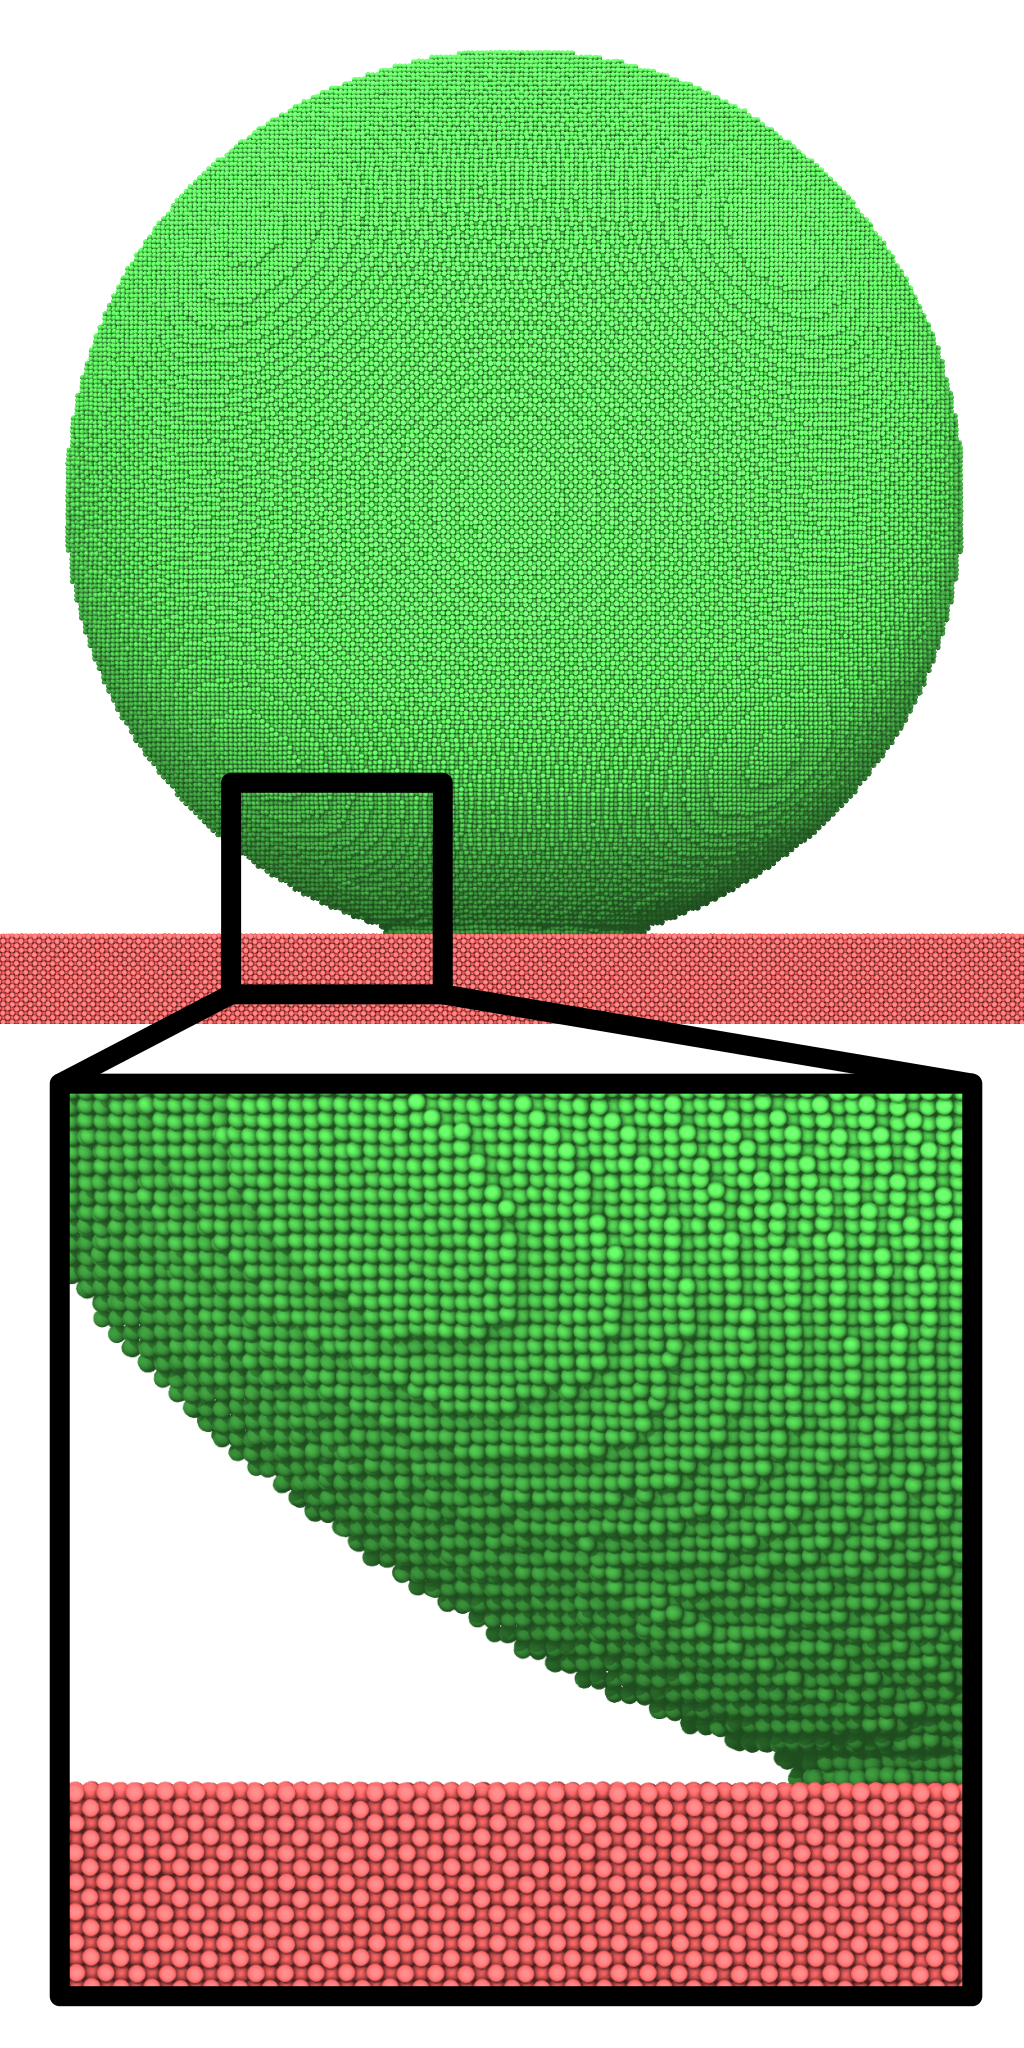
\includegraphics[width=0.85\textwidth]{single/img/equilibration/sphere_zoom_vertical.png}
			\vspace{-0.6\baselineskip}
			\caption{Fully equilibrated aluminium sphere (green) on ground (red).}
		\end{figure}
		}
	\end{column}
\end{columns}
\end{frame}


\subsection{Influence of the laser power}
\begin{frame}{Influence of the laser power - Setup}
	\begin{itemize}[<+->]
		\item Calibrating the laser power at given scanning speed % needed to melt the sample completely
		\item Picking a scanning speed
		\begin{itemize}
			\item Can be arbitrary
			\item Reasonable time for laser to pass simulation box
			\item[$\Rightarrow$] \SI{10}{\angstrom} per simulation time unit
		\end{itemize}
		\item Repeat same simulation for various laser powers
	\end{itemize}
	\vspace{2cm}
	\onslide<+->{Measure for melting rate: Common Neighbor Analysis (CNA)}
\end{frame}


\begin{frame}{Influence of the laser power - Results}
\begin{columns}
	\begin{column}{0.5\textwidth}
		\visible<2->{
		\begin{figure}
			\centering
			\captionsetup{justification=centering}
			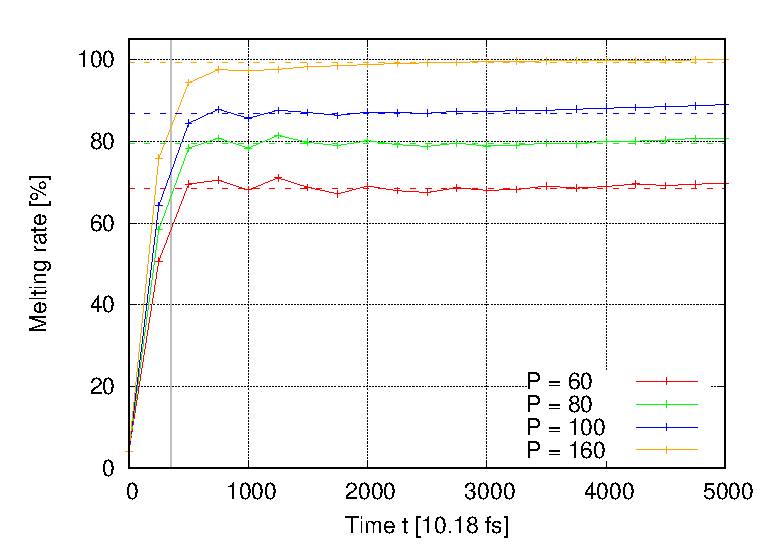
\includegraphics[width=\textwidth]{single/plt/power_calibration/cna_vel10_start_en.eps}
			\caption{short-term development}
		\end{figure}
		}
	\end{column}
	\begin{column}{0.5\textwidth}
		\visible<3->{
		\begin{figure}
			\centering
			\captionsetup{justification=centering}
			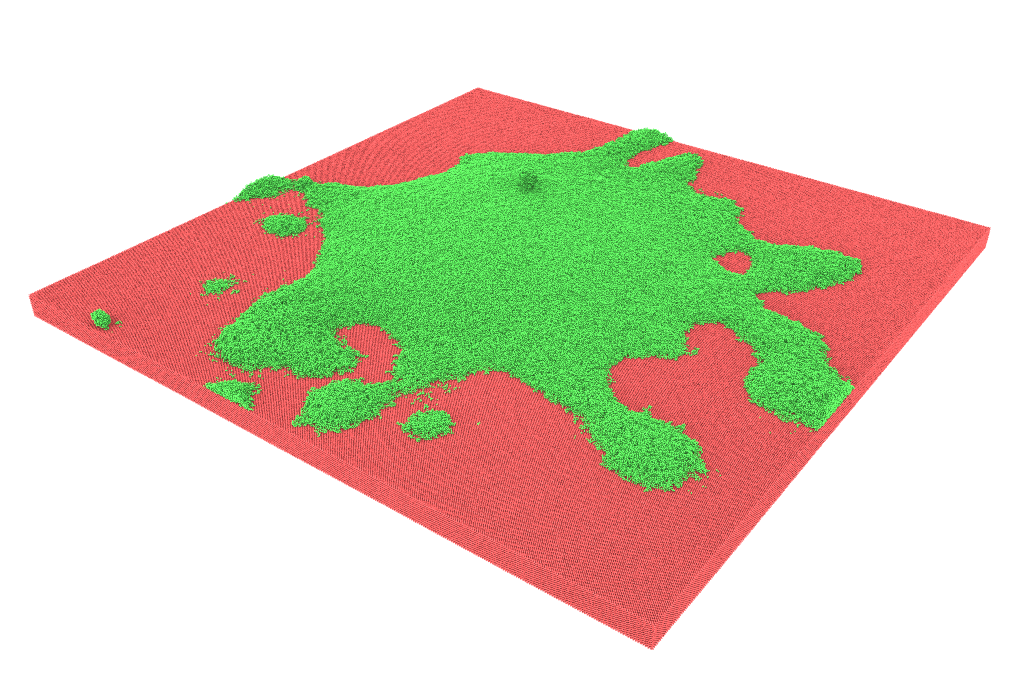
\includegraphics[width=0.815\textwidth]{single/img/power_calibration/v10_p160_c420_perspective.png}
			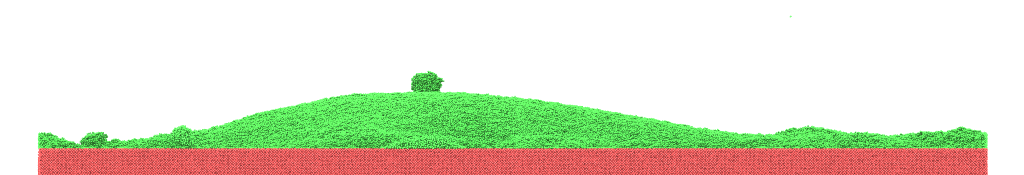
\includegraphics[width=0.815\textwidth]{single/img/power_calibration/v10_p160_c420_side_cropped.png}
			\caption{For $P = \SI{160}{\electronvolt}/\SI{10.81}{fs}$ after 21000 time units.}
		\end{figure}
		}
	\end{column}
\end{columns}
\end{frame}


\begin{frame}{Influence of the laser power - Results}
	\begin{figure}
		\centering
		\captionsetup{justification=centering}
		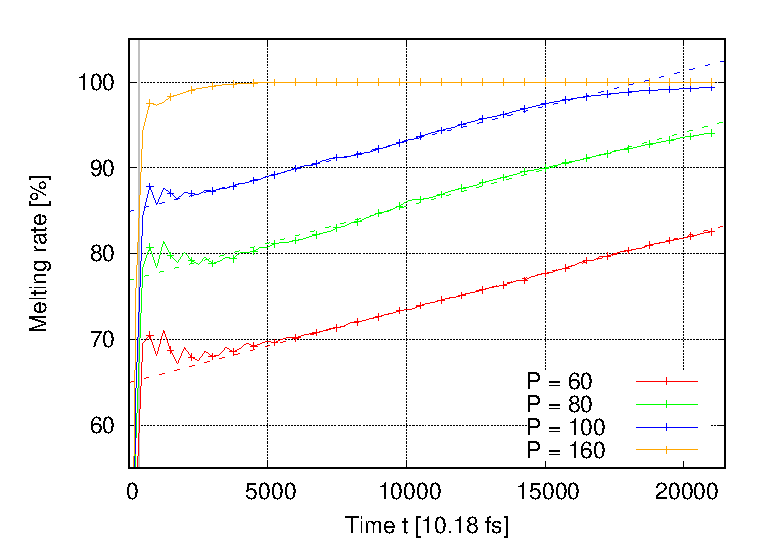
\includegraphics[width=0.5\textwidth]{single/plt/power_calibration/cna_vel10_rate_en.eps}
		\caption{long-term development}
	\end{figure}
\end{frame}


\begin{frame}{Influence of the laser power - Results}
	\begin{columns}
		\begin{column}{0.5\textwidth}
			\onslide<+->{
			\begin{figure}
				\centering
				\captionsetup{justification=centering}
				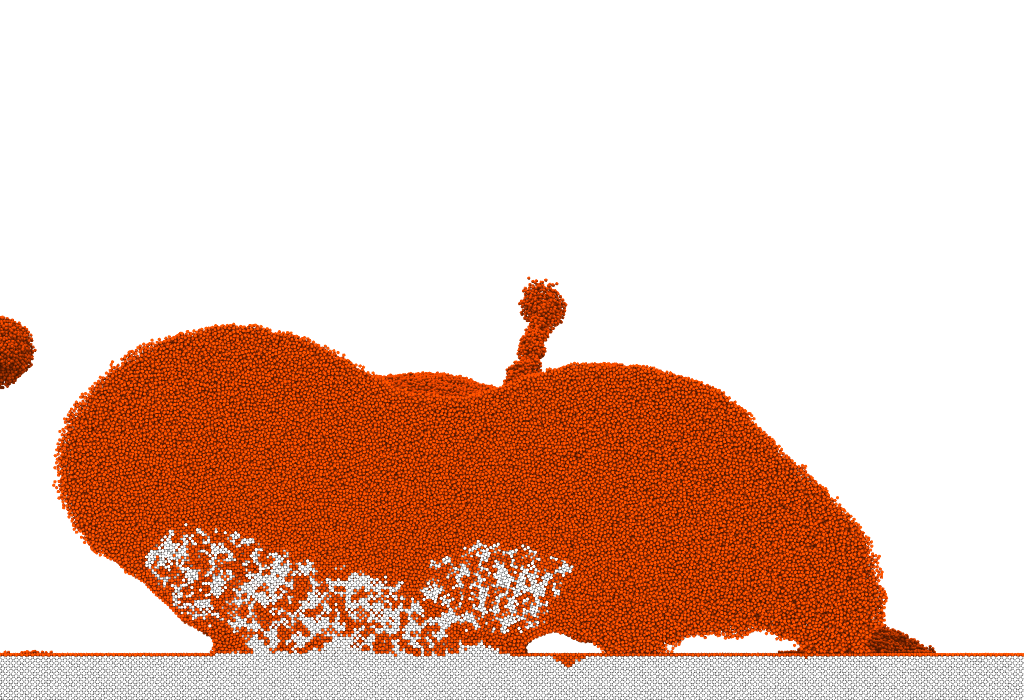
\includegraphics[width=0.95\textwidth]{single/img/power_calibration/v10_p100_c225.png}
				\caption{Cut-through after 11250 time units at $P = \SI{100}{\electronvolt}/\SI{10.81}{fs}$.}
			\end{figure}
			}
		\end{column}
		\begin{column}{0.5\textwidth}
			\onslide<+->{
			\begin{figure}
				\centering
				\captionsetup{justification=centering}
				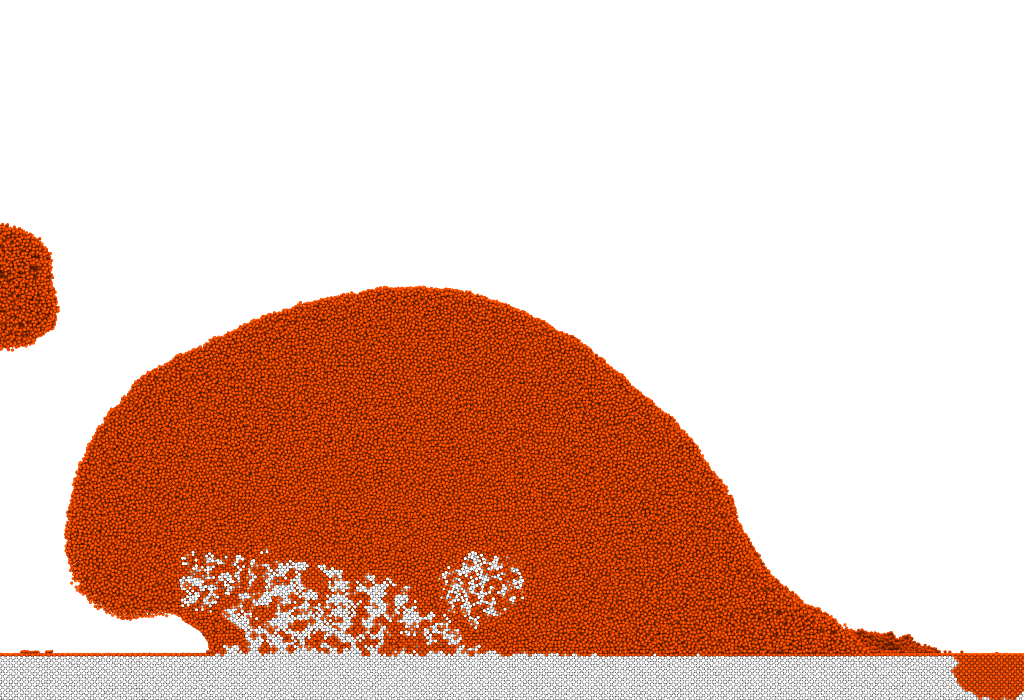
\includegraphics[width=0.95\textwidth]{single/img/power_calibration/v10_p100_c280.png}
				\caption{Cut-through after 14000 time units at $P = \SI{100}{\electronvolt}/\SI{10.81}{fs}$.}
			\end{figure}
			}
		\end{column}
	\end{columns}
	\end{frame}


\subsection{Cutting the scanning speed in half}
\begin{frame}{Cutting the scanning speed in half}
	\missing
\end{frame}
